\subsection{Zeiterfassung}
Für die Diplomarbeit sind 180 Arbeitsstuden pro Teammitglied vorgeschrieben. Um den Arbeitsaufwand jedes Teammitglieds genau festzustellen wird das Programm Clockify verwendet. Clockify ist ein kostenfreies Tool zur Zeiterfassung. Es gibt sowohl eine Desktop Applikation als auch eine Webanwendung. Clockify vereinfacht es, die Arbeitszeit zu erfassen und zu dokumentieren. Die Zeiterfassung erfolgt über die Desktop Applikation. Die Webanwendung dient zur Einsicht und Auswertung der Daten. Die Daten können in verschiedenen Formaten exportiert werden (csv, xlsx, json). Zur graphischen Darstellung der Daten wird Excel verwendet.

\textbf{Stand 31.03.2023}

\paragraph{Arbeitsaufwand der Teammitglieder}
Die folgende Abbildung und Tabelle zeigt den Arbeitsaufwand der einzelnen Teammitglieder.

\begin{table}[H]
  \centering
  \begin{tabular}{lr}
    \toprule
    \textbf{Teammitglied} & \textbf{Arbeitsaufwand} \\
    \midrule
    Joshua Lung           & 241 Stunden             \\
    Paul Hartmann         & 229 Stunden             \\
    Lukas Madlener        & 10 Stunden              \\
    \midrule
    Summe                 & 480 Stunden             \\
    \bottomrule
  \end{tabular}
  \caption{Arbeitsaufwand der Teammitglieder}
  \label{tab:zeiterfassung_teammitglieder}
\end{table}

\begin{figure}[H]
  \centering
  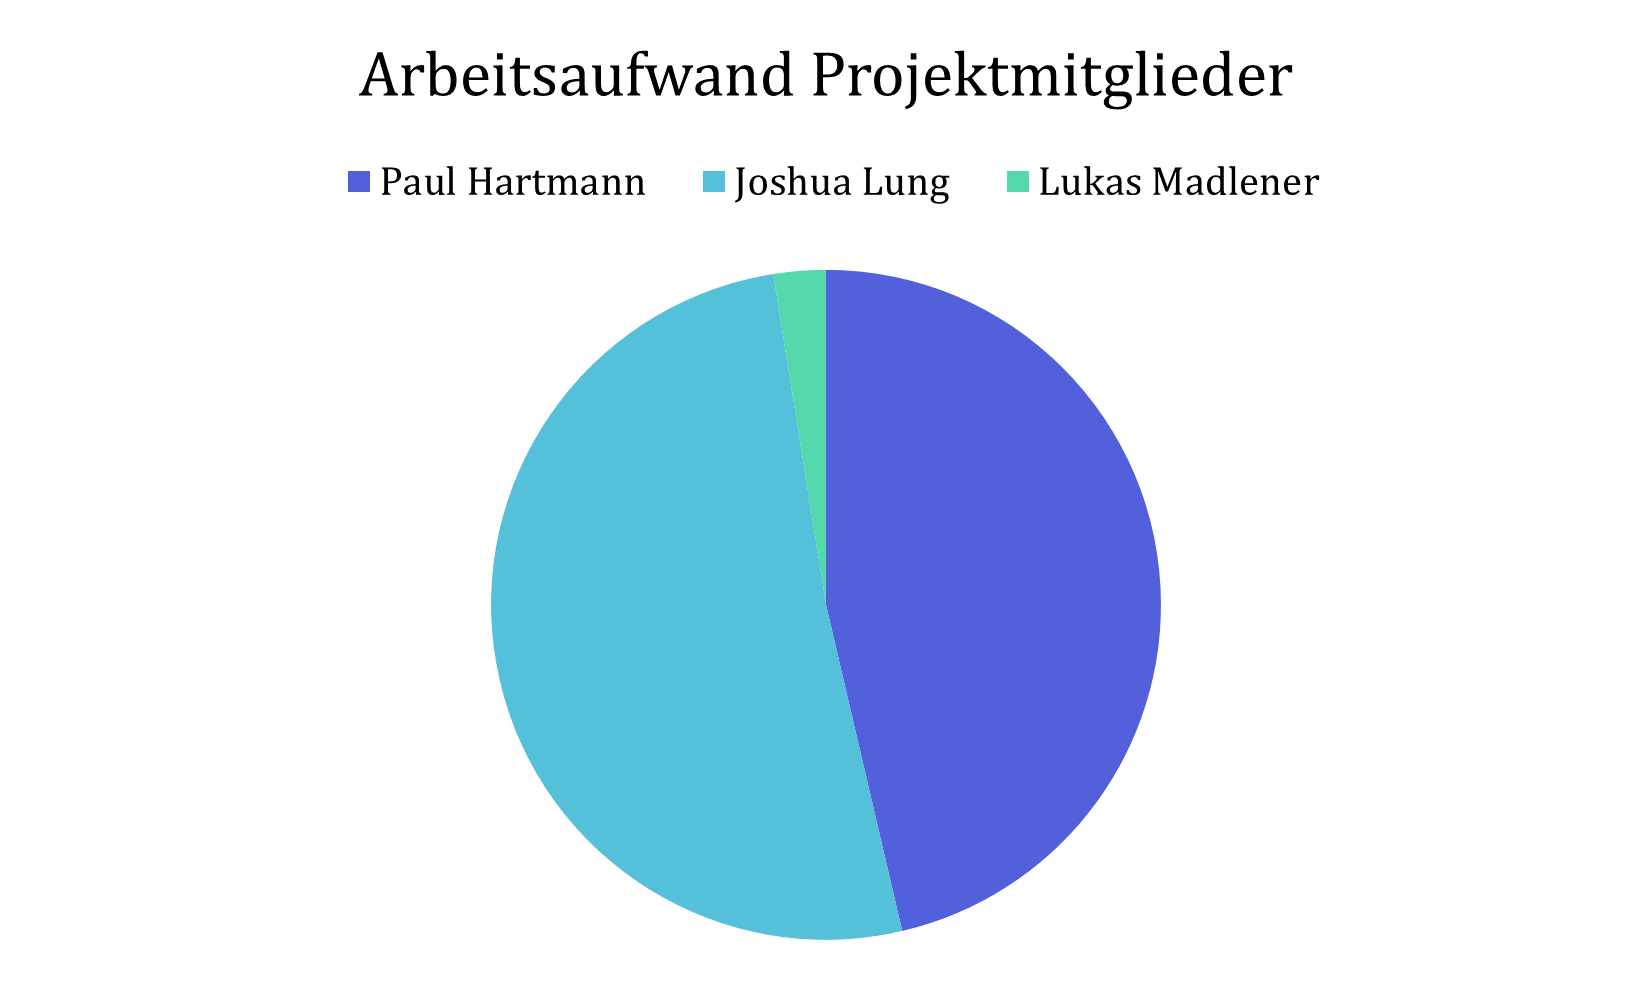
\includegraphics[width=0.8\textwidth]{images/zeiterfassung_teammitglieder.png}
  \caption{Zeitaufwand der Teammitglieder}
  \label{fig:zeiterfassung_teammitglieder}
\end{figure}


\paragraph{Arbeitsaufwand der einzelnen Projekte}
Die folgende Abbildung und Tabelle zeigen den Arbeitsaufwand der einzelnen Projekte.

\textbf{Stand 12.03.2023}

\begin{table}[H]
  \centering
  \small
  \begin{tabular}{lrrrr}
    \toprule
    \textbf{Projekt}        & \textbf{Arbeitsaufwand} & \textbf{\makecell{Paul                            \\Hartmann}} & \textbf{\makecell{Joshua\\Lung}} & \textbf{\makecell{Lukas\\Madlener}} \\
    \midrule
    Schriftliche Arbeit     & 108 Stunden             & 56 Stunden             & 51 Stunden  & 1 Stunde   \\
    Turm Controller         & 93 Stunden              &                        & 93 Stunden  &            \\
    Mobile App              & 83 Stunden              & 77 Stunden             & 6 Stunden   &            \\
    Sonstiges               & 43 Stunden              & 25 Stunden             & 16 Stunden  & 1 Stunde   \\
    Recherche               & 30 Stunden              & 13 Stunden             & 13 Stunden  & 4 Stunden  \\
    Konstruktion            & 18 Stunden              & 7 Stunden              & 7 Stunden   & 4 Stunden  \\
    Turm Physical Prototype & 16 Stunden              &                        & 16 Stunden  &            \\
    Backend (Firebase)      & 3 Stunden               & 3 Stunden              &             &            \\
    Admin Panel             & 3 Stunden               & 3 Stunden              &             &            \\
    \midrule
    Summe                   & 397 Stunden             & 184 Stunden            & 203 Stunden & 10 Stunden \\
    \bottomrule
  \end{tabular}
  \caption{Arbeitsaufwand der einzelnen Projekte}
  \label{tab:zeiterfassung_projekte}
\end{table}

\begin{figure}[H]
  \centering
  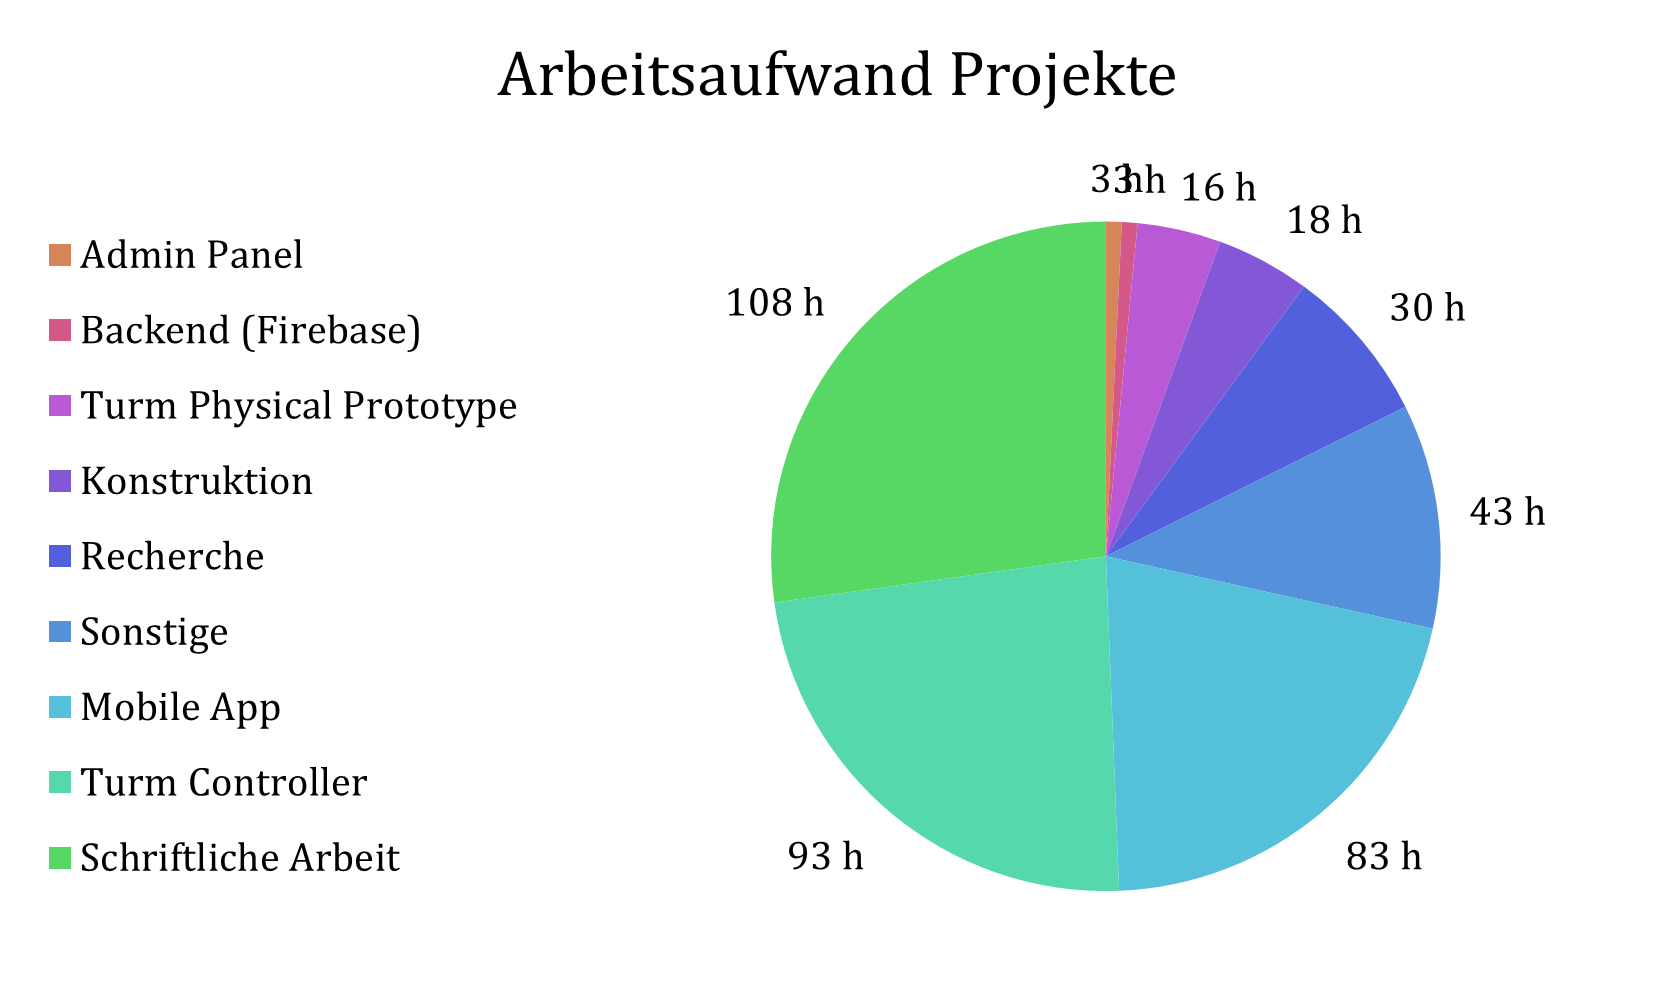
\includegraphics[width=0.8\textwidth]{images/zeiterfassung_projekte.png}
  \caption{Zeitaufwand der einzelnen Projekte}
  \label{fig:zeiterfassung_projekte}
\end{figure}